\documentclass[a4paper,dvipsnames]{article}

\input header

\title{Réseaux}

\author{}
\date{}

\begin{document}

\renewcommand{\contentsname}{}

\pagestyle{fancy}

\begin{tcolorbox}[colframe=blue!75, colback=blue!45, valign=center, height=1.5cm, top=5mm]
  \maketitle
\end{tcolorbox}

\tableofcontents

\vspace{1cm}

\thispagestyle{fancy}

\section{Notion de réseau informatique}

\subsection{Histoire}

Les réseaux existaient avant l'informatique. Un exemple notable est la
transmission optique avec des bras articulés du Français Claude Chappe au
XVIII\ieme{} siècle.

Voici deux vidéos pour l'histoire des réseaux en général:
\begin{itemize}
\item
\href{https://www.youtube.com/watch?v=LKGkmbz57ds}{Une vidéo courte donnant un bon aperçu}

\item \href{https://www.youtube.com/watch?v=0kjlITYI9Lk}{Une excellente vidéo du National Géographic qui insiste sur la
  transmission optique}

\end{itemize}

Ce qui nous intéresse ce sont les réseaux informatiques.

On sait transmettre de l'information avec de l'électricité depuis 1844, et sans
fil avec des ondes électromagnétique (ondes radios) depuis 1896 avec la
naissance de la télégraphie sans fil (TSF).

L'information est codée par la présence ou non d'un signal (un voltage sur le
fil). Avec les ordinateurs qui apparaissent dans les années 1950, le problème
est de faire communiquer plusieurs ordinateurs en les reliant sur un même
réseau, ce qui suppose plusieurs choses:
\begin{itemize}
  \item L'établissement de protocoles pour que tous les ordinateurs parlent le
    même langage sur le réseau.
  \item La mise au point d'un système d'adresses et de routage pour orienter les
    messages vers leur destinataire final.
\end{itemize}

\smallskip

Pour les protocoles,
le principe de la {\color{red}transmission de paquets} est introduit par Paul Baran et Davies en 1961 : il consiste à découper les données en paquets, ce qui permet de transmettre avec un débit variable (un courriel nécessite l'envoi ponctuel de petits paquets alors que pour transférer un fichier, il faut envoyer rapidement de gros paquets).

\smallskip

{\color{red}Arpanet}, le projet de réseau interuniversitaire financé par l'Arpa (agence de recherche de la défense américaine) , voit le jour en 1969 sous la direction de Leonard Kleinrock : les données sont découpées en paquets, transmis en séquence les uns à la suite des autres.

\smallskip

Le routage apparaît dans les années 70: Louis Pouzin, après un séjour au MIT, développe en France le réseau {\color{red}Cyclades} qui est le premier véritable réseau à {\color{red}commutation de paquets} : les paquets transitent de façon indépendante dans le réseau grâce à un protocole qui préfigure Internet Protocol puis sont remis en l'ordre à l'arrivée. Le circuit des paquets est donc variable contrairement à la {\color{red}commutation de circuits} implémentée dans le réseau téléphonique.

\smallskip

Aux États-Unis, Vinton Cerf et Robert Kahn s'inspirent des idées de Pouzin et
inventent les protocoles {\color{red}IP} et {\color{red}TCP}. C'est ce protocole
(en version 4 (1982) et 6 (1995)) qui est encore utilisé de nos jours pour coder l'information
et acheminer les messages à leur destination. L'interconnexion des réseaux
Arpanet et Csnet en 1983 avec {\color{red}TCP/IP} marque la naissance d'Internet
et son expansion au niveau mondial dans les sphères universitaires et de la
recherche.

\smallskip

En 1989, Tim Berners-Lee invente le {\color{red}Web} qui est une application de documents hypertextes s'exécutant par-dessus le réseau {\color{red}Internet}. L'ouverture des protocoles Web au grand public en 1993 connaît un succès fulgurant, d'autres services Internet comme le mail ou le transfert de fichier de pair à pair se popularisent aussi. Le trafic Internet explose : de quelques mégabits par seconde en 1992, on est passé à près de 100 térabits par seconde en 2018 avec près de 3,2 milliards d'internautes en 2016.

\subsection{Terminologie et classification des réseaux}

\begin{definition}[breakable]{terminologie}{}
 \begin{enumerate}
   \item Un {\color{red}réseau} est un ensemble de noeuds reliés par des liens et correspond mathématiquement à un graphe. Dans un {\color{red}réseau informatique} les noeuds ou hôtes sont des équipements informatiques comme des ordinateurs, des routeurs... et les liens peuvent être variés selon la technologie utilisée : filaire (Ethernet,...) ou par ondes (Wifi,...).
   \item Une {\color{red}interface} est le point de raccordement, matériel (carte réseau) ou logiciel, entre un lien et un noeud.
   \item Un {\color{red}protocole} est un ensemble de règles permettant d'établir une communication entre deux noeuds du réseau et de garantir éventuellement certains services (fiabilité, confidentialité...)
   \item Un {\color{red}service réseau} est une application capable de communiquer en réseau et proposant des fonctionnalités. Par exemple, un service Web peut fournir des pages Web au navigateur d'un client. Sur un réseau pédagogique de lycée, un service de gestion et de partage de fichiers permet aux utilisateurs d'accéder à leurs fichiers depuis n'importe quel machine cliente.
   \item Un {\color{red}serveur} désigne un matériel ou un logiciel exécutant un {\color{red}service réseau}. Il fournit un service à des {\color{red}clients} selon une {\color{red}architecture client/serveur}. Pour une présentation de l'architecture client-serveur, on pourra visionner cette \href{https://vimeo.com/138623558}{vidéo}.

     \begin{center}
       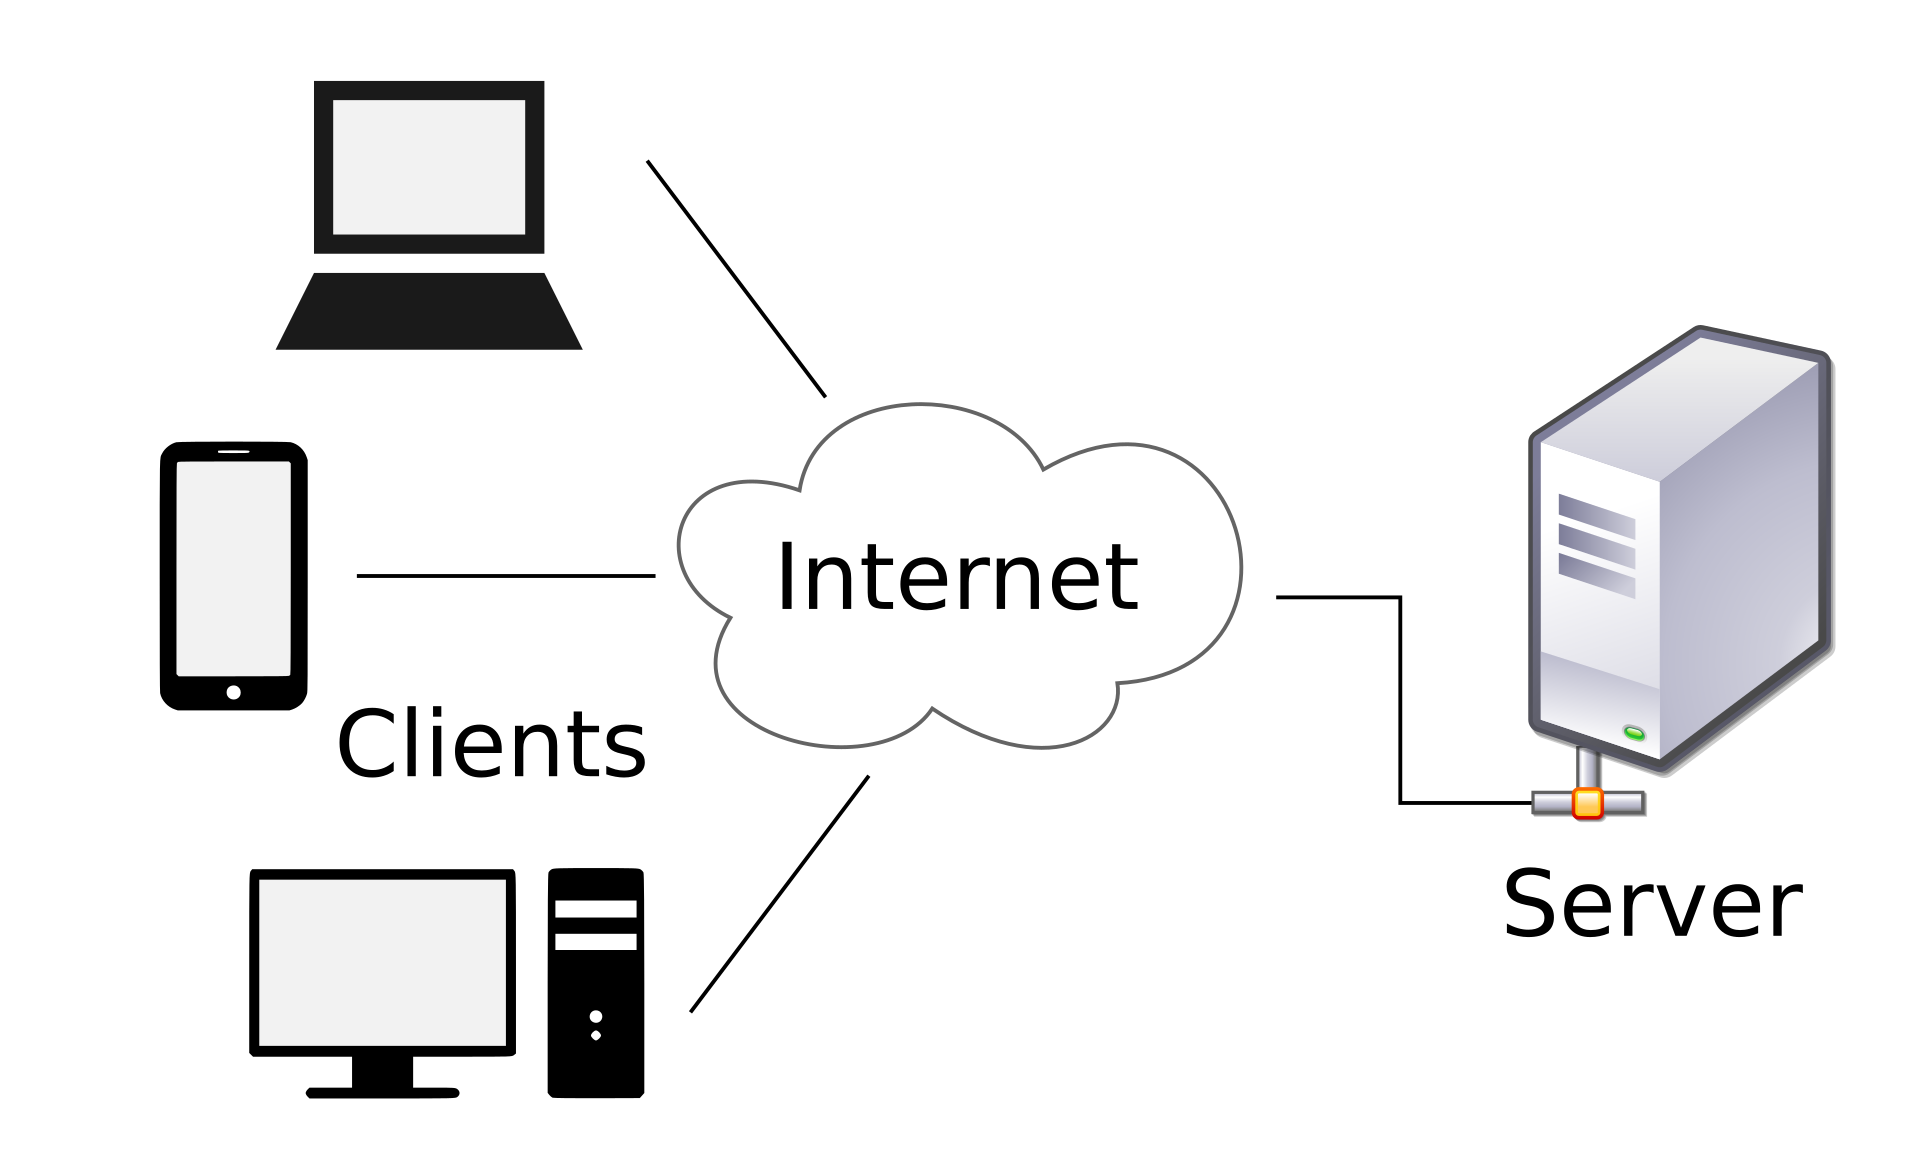
\includegraphics[width=6cm]{img/architecture_client-serveur.png}
     \end{center}
 \end{enumerate}
\end{definition}

\medskip

\begin{definition}[breakable]{classification des réseaux}{}
 \begin{enumerate}
   \item Les réseaux informatiques peuvent être de différentes tailles :
     \begin{itemize}
       \item les réseaux locaux ou {\color{red}Local Area Network (LAN)} limités à une zone géographique restreinte (maison, entreprise, lycée...)
     \item les réseaux étendus ou {\color{red}Wide Area Network (WAN)} couvrant de vastes zones géographiques (pays, continent ). Ce sont, par exemple, les réseaux des fournisseurs d'accès internet (Free, Orange, SFR...), de grandes sociétés...
     \end{itemize}
     Internet est une interconnexion mondiale de réseaux.
   \item Les réseaux informatiques utilisent des liens de technologies diverses :
     \begin{itemize}
       \item des {\color{red}liaisons filaires} : câbles en cuivre à paires torsadées, fibres optiques ...
       \item des liaisons {\color{red}par ondes} : Wifi, Bluetooth, satellite,
         parabole entre deux antennes (Rangiroa et Tikehau), 4G...
     \end{itemize}
   \item L'interconnexion dans l'Internet de tous ces réseaux hétérogènes sur le plan matériel a été rendu possible par le développement de protocoles logiciels. Pour une présentation globale d'Internet, on pourra visionner cette \href{https://www.youtube.com/watch?v=dCknqcjcItU}{vidéo}.

     \begin{center}
       \fbox{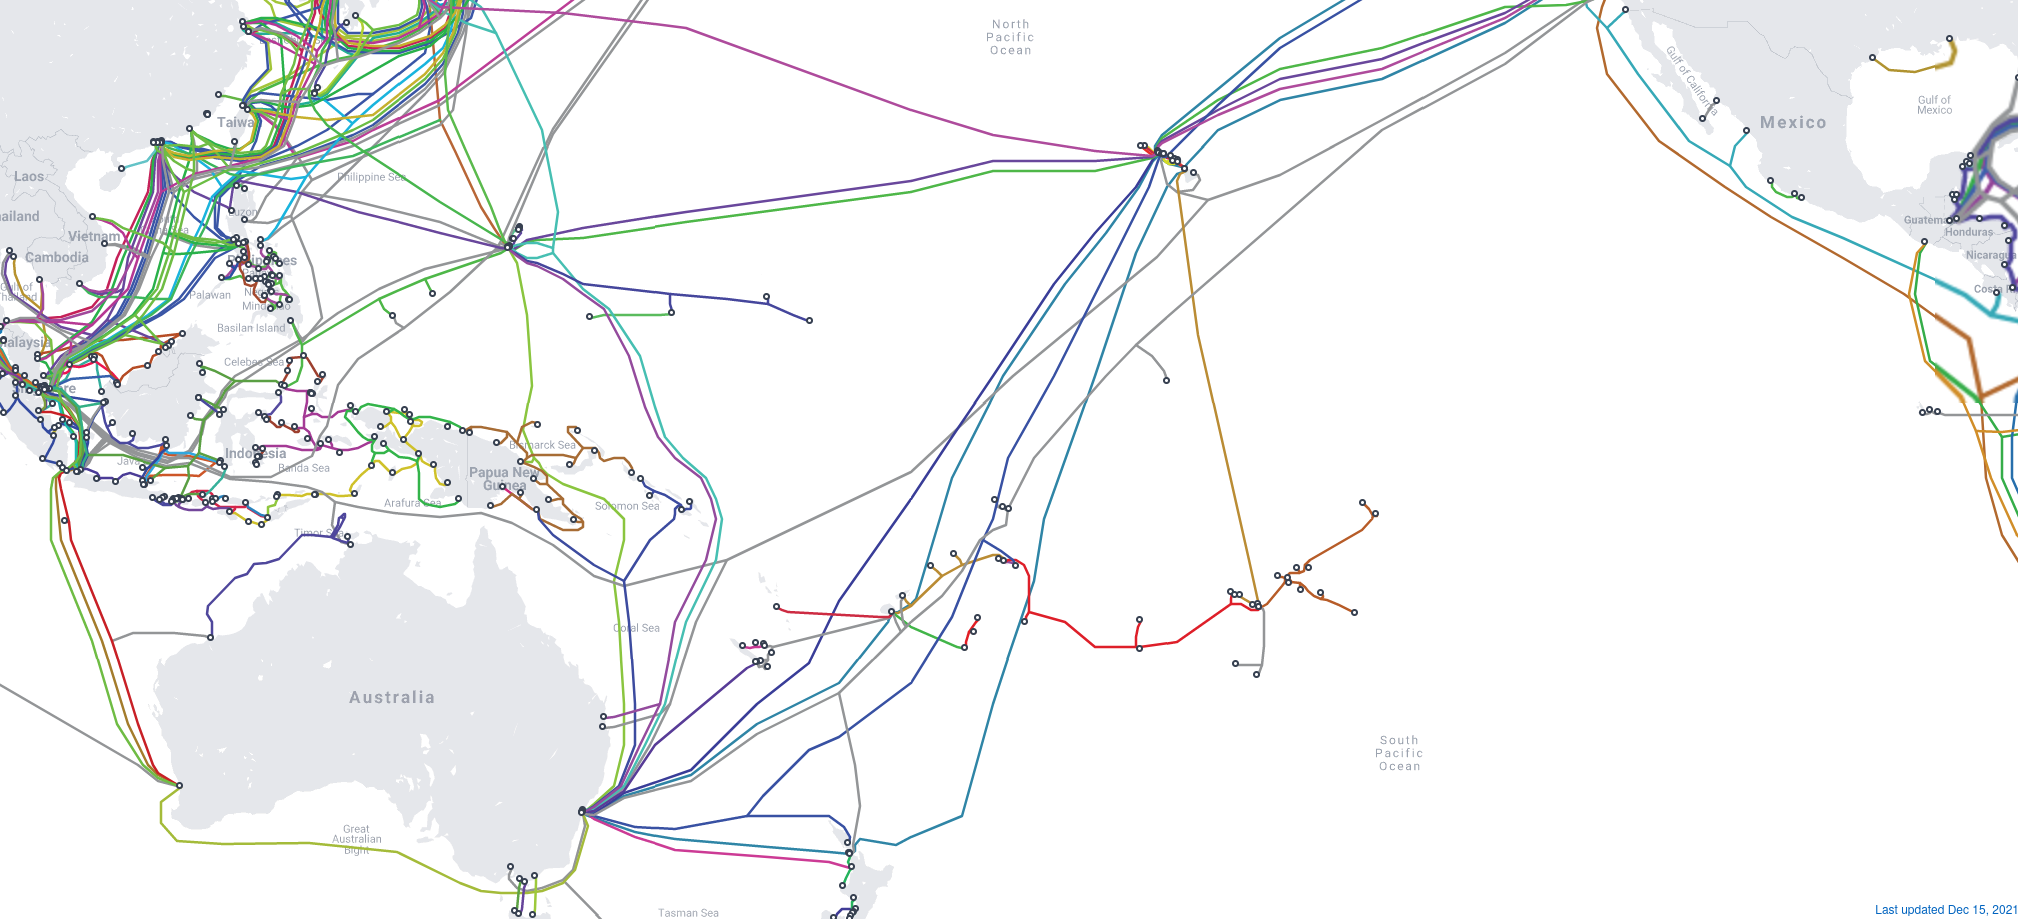
\includegraphics[width=12cm]{img/carte_cables_sous-marins.png}}

       \smallskip

       \scriptsize\textit{Carte des câbles sous-marins -- \url{https://www.submarinecablemap.com/}}
     \end{center}

 \end{enumerate}
\end{definition}

\smallskip

\begin{exercice}{QCM type E3C}{}
 \begin{enumerate}
   \item Un protocole est un ensemble de...
     \begin{enumerate}
       \item matériels connectés entre eux
       \item serveurs et de clients connectés entre eux
       \item règles qui régissent les échanges entre équipements informatiques
       \item règles qui régissent les échanges entre un système d'exploitation et les applications
     \end{enumerate}
   \item Comment s'appelle l'ensemble des règles qui régissent les échanges sur Internet ?
     \begin{enumerate}
       \item les couches
       \item le wifi
       \item les protocoles
       \item les commutateurs
     \end{enumerate}
   \item L'architecture client-serveur :
     \begin{enumerate}
       \item est un mode de communication entre programmes
       \item est une architecture matérielle de coopération entre machines
       \item est un mode de communication entre routeurs
       \item est un mode de communication entre commutateurs
     \end{enumerate}
 \end{enumerate}
\end{exercice}

\pagebreak

\section{Architecture d'un réseau}

\subsection{Adresse MAC et IP}

Sur le réseau physique, c'est-à-dire le même switch ethernet, ou la même antenne
wifi, les machines s'échangent
des paquets en utilisant les adresses MAC. Sur un réseau plus grand, dès que
l'on
doit passer par un routeur, et en particulier sur l'internet mondial, on utilise
une adresse IP.

\begin{definition}[breakable]{adresse MAC}{}
  Chaque interface sur le réseau dispose d'une adresse MAC qui est une valeur
  unique attribuée à la carte réseau (Ethernet, Wifi, 4G, 5G, ...) lors de sa
  fabrication en usine, ou changée plus tard (voir plus bas).

  \smallskip

  Cette adresse est codée sur 48 bits (présentés sous la forme de 6 octets en
  hexadécimal), par exemple \texttt{fc:aa:14:75:45:a5}. Les trois premiers
  octets correspondent au code du fabricant. Un site comme
  \url{https://www.macvendorlookup.com/} permet de retrouver le fabricant d'une
  adresse MAC quelconque.

  Les adresses MAC sont souvent utilisées pour autoriser des machines spécifiques
  (laptop ou téléphone) à utiliser un réseau... mais on peut changer les
  adresses MAC avec la plupart des cartes réseaux modernes et les téléphones et
  tablettes utilisent aujourd'hui par défaut des adresses MAC aléatoires qui
  changent périodiquement. Tout ceci pause souvent des problèmes de connexions.
\end{definition}

\begin{definition}[breakable]{adresse IP}{}
  Une adresse IP est aussi une valeur unique attribuée à chaque interface.  Elle
  est sur 32 bits en IPV4 (version 4 de IP) et sur 128 bits en IPV6.

  On écrit en général les adresses IPV4 en groupant les 32 bits en 4 octets que
  l'on donne en décimal. Ex: 192.168.0.1. Une adresse IPV6 s'écrit avec 8 paquets de
  16 bits en héxadécimal, avec omission des zéros consécutifs au milieu.
  Ex: fe80::42:2dff:fe26:1c7f signifie fe80:0000:0000:0000:0042:2dff:fe26:1c7f.

  La relation entre le nom d'une machine (ex: google.com) et sa (ou ses)
  adresses IP (142.250.68.46 ou 2607:f8b0:4007:810::200e pour google.com, le
  jour où ce document a été écrit)
  est la
  charge des serveurs de noms (DNS: Domain Name Server), et le passage de
  l'adresse IP à l'adresse MAC est géré par le protocole ARP (Address Resolution
  Protocol). ARP ne
  nécessite en général pas de configuration.
\end{definition}

  Le réseau internet mondial connait depuis les années 2000 une pénurie
  d'adresse IPV4 (il n'y en a que 4 milliards environ) et le passage global à
  IPV6 qui est un standard accepté par les autorités depuis 1998 se fait
  attendre ...  Cette pénurie rend impossible d'assigner une adresse visible
  mondialement à toutes les machines du monde. On utilise alors des redirections
  de ports et autres techniques pour accéder aux machines d'un réseau local qui
  n'ont pas d'IP connue à l'extérieur. Cela complexifie la tâche des
  administrateurs et diminue les performance du réseau.

  IPV6 simplifie énormément les choses car les 48bits de droites de l'IPV6 sont
  l'addresse MAC, les 64 bits de droites (donc l'addresse MAC + 16 bits) sont
  l'adresse sur le réseau local et les 64 bits de gauche l'adresse du réseau
  local lui même. On dispose ainsi potentiellement de 16 milliards de milliards
  d'adresses pour les réseaux locaux et autant pour le nombre de machines sur
  chaque réseau. IPV6 rendrait par exemple beaucoup plus facile le jeu en réseau!

\medskip

\subsection{Un premier réseau local}

\begin{activite}[breakable]{}{}
  \begin{enumerate}
    \item À l'aide du logiciel \href{https://www.lernsoftware-filius.de/Herunterladen}{Filius}, créer le réseau local ci-dessous :

      \begin{center}
	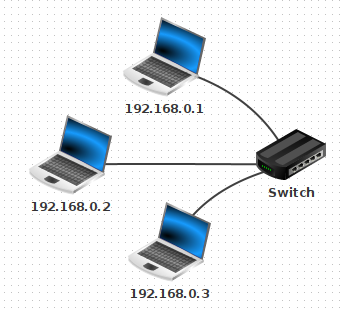
\includegraphics[width=6cm]{img/f1.png}
      \end{center}

    \item Tester alors le \mintinline{bash}{ping} de la machine \texttt{192.168.0.1} vers la machine \texttt{192.168.0.3}.

      \begin{center}
	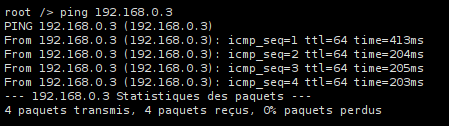
\includegraphics[width=8cm]{img/ft1.png}
      \end{center}
  \end{enumerate}
\end{activite}

\medskip


\begin{definition}[breakable]{différences entre switch (ou commutateur) et hub}{}
 \begin{enumerate}
   \item Au sein d'un {\color{red}hub Ethernet} (de moins en moins vendus), il n'y a aucune analyse des données qui transitent : il s'agit simplement d'un dédoublement des fils de cuivre (tout comme une multiprise électrique). L'intégralité des messages est donc envoyée à l'intégralité des ordinateurs du réseau, même s'ils ne sont pas concernés.

     \begin{center}
       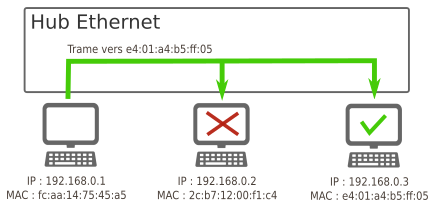
\includegraphics[width=8cm]{img/hub.png}
     \end{center}

   \item Au sein d'un {\color{red}switch Ethernet} , une analyse est effectuée sur la trame qui est à distribuer. Lors du branchement d'un nouvel ordinateur sur le switch, celui-ci récupère son adresse MAC, ce qui lui permet de trier les messages et de ne les distribuer qu'au bon destinataire.

     \begin{center}
       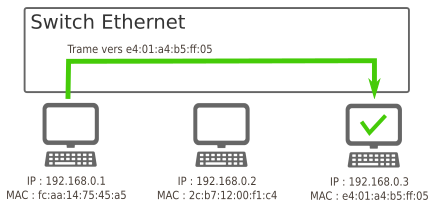
\includegraphics[width=8cm]{img/switch.png}
     \end{center}
 \end{enumerate}
\end{definition}

\subsection{Un deuxième sous-réseau}

\begin{activite}[breakable]{}{}
  \begin{enumerate}
    \item Ajouter un deuxième sous-réseau (penser à bien renommer les switchs) :
      \begin{center}
	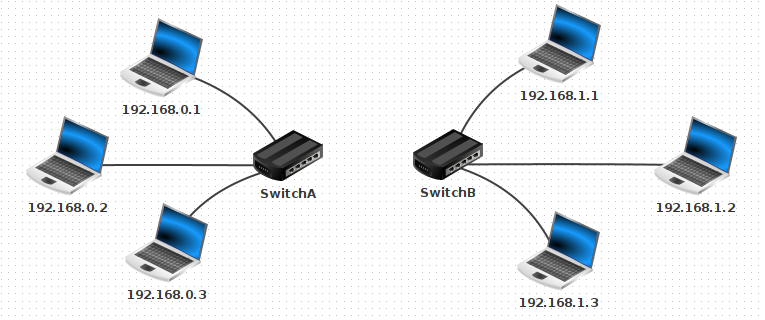
\includegraphics[width=10cm]{img/f2.png}
      \end{center}
    \item Relier ces deux sous-réseaux à l'aide d'un câble :
      \begin{center}
	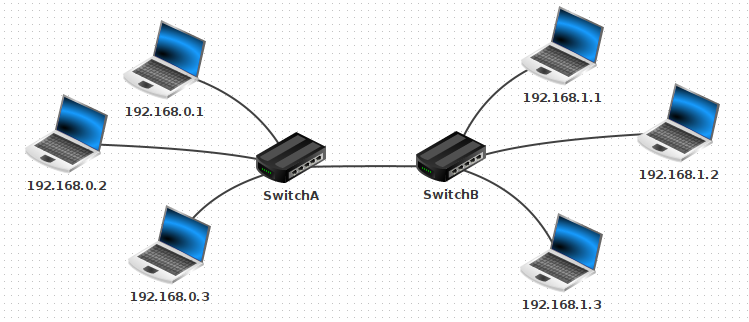
\includegraphics[width=10cm]{img/f3.png}
      \end{center}
      \begin{enumerate}
	\item Essayer de \og{}pinger\fg{} la machine \texttt{192.168.1.2} depuis la machine \texttt{192.168.0.1}. Que se passe-t-il ?
	\item Temporairement, changer l'adresse IP de la machine \texttt{192.168.1.2} en \texttt{192.168.0.33} puis essayer à nouveau le ping depuis la machine \texttt{192.168.0.1}.
      \end{enumerate}
  \end{enumerate}
\end{activite}

\medskip

\begin{remarque*}[breakable]{}{}
  Dans le premier cas, le ping n'aboutissait pas car les machines \texttt{192.168.1.2} et \texttt{192.168.0.1} ne sont pas dans le même sous-réseau. Dans le second cas, le ping aboutit car les machines \texttt{192.168.0.1} et \texttt{192.168.0.3} sont dans le même sous-réseau.

  \medskip

  Comment savoir si deux machines sont dans le même sous-réseau ?
\end{remarque*}

\medskip

\begin{methode}[breakable]{explication basique}{}
  Dans Filius, lors de l'attribution de l'adresse IP à une machine, une ligne nous permet de spécifier le {\color{red}masque de sous-réseau} (appelé simplement \og{}Masque\fg{} dans Filius). C'est ce masque qui va permettre de déterminer si une machine appartient à un sous-réseau ou non, en fonction de son adresse IP.

  \begin{center}
    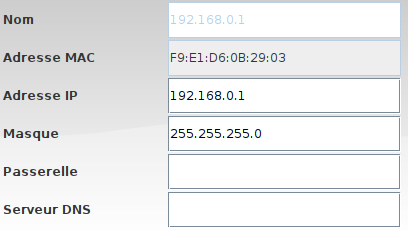
\includegraphics[width=6cm]{img/f4.png}
  \end{center}

  \begin{itemize}
    \item Avec comme masque \texttt{255.255.255.0}, toutes les machines ayant une adresse IP commençant par les trois mêmes premiers nombres appartiendront à un même sous-réseau. Comme ceci est le réglage par défaut de Filius, cela explique pourquoi \texttt{192.168.0.33} et \texttt{192.168.0.1} sont sur un même sous-réseau, et pourquoi \texttt{192.168.1.2} et \texttt{192.168.0.1} ne sont pas sur un même sous-réseau.

      Dans cette configuration, 256 machines peuvent donc appartenir au même sous-réseau (ce n'est pas tout à fait le cas car des adresses finissant par 0 ou par 255 sont réservées).

    \item Avec comme masque \texttt{255.255.0.0}, toutes les machines ayant une adresse IP commençant par les deux mêmes premiers nombres appartiendront à un même sous-réseau.

      Dans cette configuration, $\np{65536}$ machines peuvent être dans le même sous-réseau (car $256^2=~\np{65536}$).
  \end{itemize}
\end{methode}

\medskip

\begin{activite}[breakable]{}{}
  \begin{enumerate}
    \item Renommer \texttt{192.168.0.33} en \texttt{192.168.1.2} et modifier son masque en \texttt{255.255.0.0}.
    \item Modifier aussi le masque de \texttt{192.168.0.1} en \texttt{255.255.0.0}.
    \item Avec ces modifications, que peut-on dire du ping de \texttt{192.168.0.1} vers \texttt{192.168.1.2} ? Vérifier votre réponse.
  \end{enumerate}
\end{activite}

\medskip

\begin{methode}[breakable]{explication \og{}avancée\fg{}}{}
 Lorsqu'une machine A veut envoyer un message à une machine B, elle doit déterminer si cette machine :
 \begin{itemize}
   \item appartient au même sous-réseau, auquel cas le message est envoyé directement via un ou plusieurs switchs ;
   \item n'appartient pas au même sous-réseau, auquel cas le message doit d'abord transiter par un routeur.
 \end{itemize}

 En notant \mintinline{bash}{IP_A} et \mintinline{bash}{IP_B} les adresses IP respectives des machines A et B, et \mintinline{bash}{M} le masque de sous-réseau :

 \begin{center}
   A et B appartiennent au même sous-réseau si, et seulement si, \mintinline{bash}{IP_A & M = IP_B & M}.
 \end{center}
\end{methode}

\medskip

\begin{exercice}[breakable]{}{}
  Compléter le tableau suivant et déterminer quelles machines font partie d'un même sous-réseau :

  \begin{center}
    \begin{tabular}{@{}cccc@{}}
     & Machine A & Machine B & Machine C\\
     \toprule
      \mintinline{bash}{IP} & \texttt{192.168.129.10} & \texttt{192.168.135.200} & \texttt{192.168.145.1}\\[2pt]
      \mintinline{bash}{M} & \texttt{255.255.248.0} & \texttt{255.255.248.0} & \texttt{255.255.248.0}\\[2pt]
      \mintinline{bash}{IP & M} & & &\\
      % correction
      % \mintinline{bash}{IP & M} & \mintinline{bash}{192.168.128.0} & \mintinline{bash}{192.168.128.0} & \mintinline{bash}{192.168.144.0}
    \end{tabular}
  \end{center}
\end{exercice}

\medskip

\begin{definition}[breakable]{notation CIDR}{}
  D'après ce qui précède, 2 informations sont nécessaires pour déterminer le sous-réseau auquel appartient une machine : son IP et le masque de sous-réseau. Une convention de notation permet d'écrire simplement ces deux renseignements : la notation CIDR.
  \tcblower
  Une machine d'IP \texttt{192.168.0.33} avec un masque de sous-réseau \texttt{255.255.255.0} sera désignée par \texttt{192.168.0.33/24} en notation CIDR.

  Le suffixe \texttt{/24} signifie que le masque de sous-réseau commence par 24 bits consécutifs de valeur 1 : le reste des bits (donc 8 bits) est mis à 0.
  Autrement dit, ce masque vaut \texttt{11111111.11111111.11111111.00000000} , soit \texttt{255.255.255.0}.
\end{definition}

\medskip

\begin{exercice}[breakable]{}{}
  De la même manière, déterminer les masques correspondant aux suffixes \texttt{/16} et \texttt{/21}.
  % correction
  % De la même manière, le suffixe / 16 donnera un masque de 11111111.11111111.00000000.00000000 , soit 255.255.0.0.
  % Ou encore, un suffixe / 21 donnera un masque de 11111111.11111111.11111000.00000000 , soit 255.255.248.0.
\end{exercice}

\subsection{Nécessité d'un routeur}

La solution initiale (relier les deux switchs par un cable pour unifier les deux sous-réseaux) n'est pas viable à l'échelle d'un réseau planétaire.

\smallskip

Pour que les machines de deux réseaux différents puissent être connectées, on va utiliser un dispositif équipé de deux cartes réseaux situé à cheval entre les deux sous-réseaux. Cet équipement de réseau est appelé routeur.

\begin{center}
  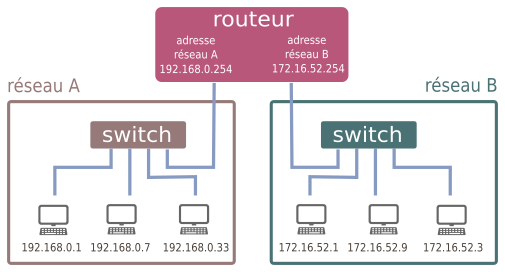
\includegraphics[width=9cm]{img/routeur.png}
\end{center}

\begin{proposition}[breakable, title=Principe de fonctionnement d'un routeur]{}{}
  Imaginons que la machine \texttt{192.168.0.1/24} veuille communiquer avec la machine \texttt{172.16.52.3/24}.

  \smallskip

  L'observation du masque de sous-réseau de la machine \texttt{192.168.0.1/24} nous apprend qu'elle ne peut communiquer qu'avec les adresses de la forme \texttt{192.168.0.X/24}, où \texttt{X} est un nombre entre 0 et 255.

  \tcblower

  Voici les 3 étapes du routage :

  \begin{enumerate}
    \item Lorsque qu'une machine A veut envoyer un message à une machine B, elle va tout d'abord vérifier si cette machine appartient à son réseau local. Si c'est le cas, le message est envoyé par l'intermédiaire du switch qui relie les deux machines.
    \item Si la machine B n'est pas trouvée sur le réseau local de la machine A, le message va être acheminé vers le routeur par l'intermédiaire de son adresse de passerelle (qui est bien une adresse appartenant au sous-réseau de A).
    \item De là, le routeur va regarder si la machine B appartient au deuxième sous-réseau auquel il est connecté. Si c'est le cas, le message est distribué, sinon, le routeur va donner le message à un autre routeur auquel il est connecté et va le charger de distribuer ce message : c'est le procédé (complexe) de routage qui sera vu en classe de Terminale.
  \end{enumerate}

  Dans notre exemple, l'adresse \texttt{172.16.52.3} n'est pas dans le sous-réseau de \texttt{192.168.0.1}. Le message va donc transiter par le routeur.

  \begin{center}
    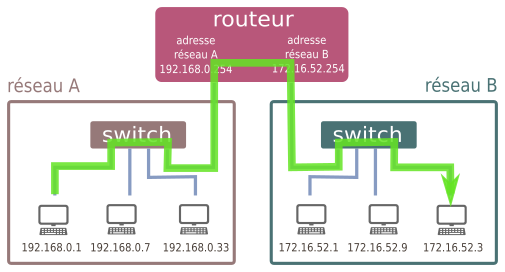
\includegraphics[width=9cm]{img/routeur2.png}
  \end{center}
\end{proposition}

\medskip

\begin{activite}[breakable]{illustration avec Filius}{}
  \begin{enumerate}
    \item Ajouter un routeur entre le \texttt{SwitchA} et le \texttt{SwitchB}.
      \begin{center}
	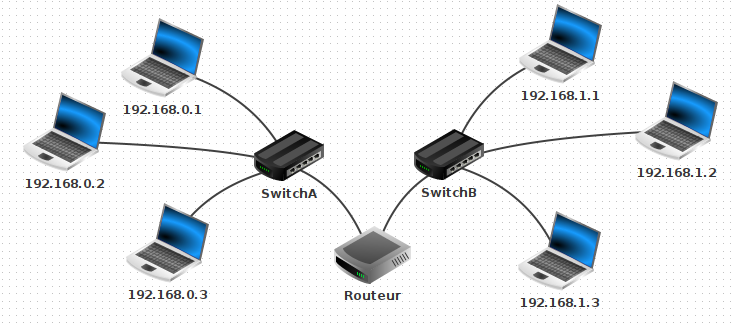
\includegraphics[width=10cm]{img/f5.png}
      \end{center}
    \item Configurer le routeur de la façon suivante :
      \begin{enumerate}
	\item adresse \texttt{192.168.0.254} pour l'interface reliée au \texttt{SwitchA} ;
	\item adresse \texttt{192.168.1.254} pour l'interface reliée au \texttt{SwitchB} ;
	\item dans l'onglet \verb|Général|, sélection \og{}Routage automatique\fg{}.
	  \begin{center}
	    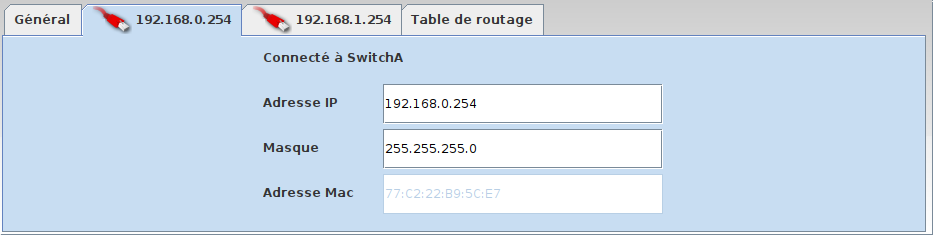
\includegraphics[width=12cm]{img/flsrouteur.png}
	\end{center}
	Ainsi configuré, le routeur peut jouer le rôle de passerelle entre les deux sous-réseaux.
    \end{enumerate}
  \item Essayer le ping entre \texttt{192.168.0.1} et \texttt{192.168.1.2}.
  \item Configurer correctement la passerelle des deux machines précédentes, et essayer à nouveau.
  \item Effectuer un \texttt{traceroute} entre les deux machines.
  \end{enumerate}
\end{activite}

\medskip

\begin{remarque}[breakable, title=Cas d'un réseau domestique]{}{}
  Dans le cas d'un réseau domestique, la box de l'opérateur joue simultanément le rôle de switch et de routeur :
  \begin{itemize}
    \item switch car elle répartit la connexion entre les différents dispositifs (ordinateurs branchés en ethernet, smartphone en wifi, tv connectée...) ;
    \item routeur car elle fait le lien entre ce sous-réseau domestique (les appareils de votre maison) et le réseau Internet.
  \end{itemize}

  \begin{center}
    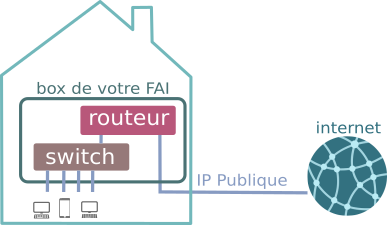
\includegraphics[width=8cm]{img/boxmaison.png}
  \end{center}
\end{remarque}

\medskip

\begin{definition}[breakable, title=Les commandes ipconfig (Windows) et ip (Linux)]{}{}
  Les commandes \texttt{ifconfig} ou \texttt{ip address} sous Linux ou \texttt{ipconfig} sous Windows permettent d'afficher les adresses physique (MAC) ou logique (IP) d'une interface réseau.
\end{definition}

\medskip

\begin{exercice}[breakable]{}{}
  Voici par exemple ce que donne \texttt{ip adress} :

  \begin{center}
    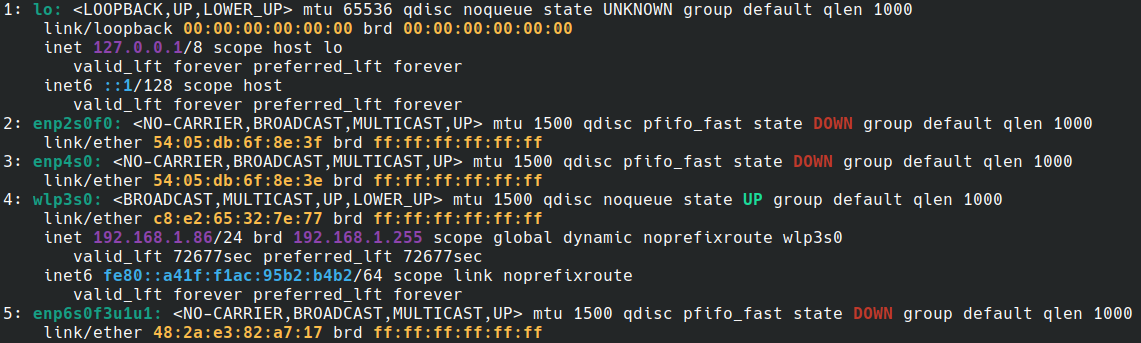
\includegraphics[width=14cm]{img/ip_address.png}
  \end{center}

  Lire l'adresse MAC et l'adresse IP de l'interface \texttt{wlp3s0}.
\end{exercice}

\medskip

\begin{activite}[breakable]{serveur web}{}
  \begin{enumerate}
    \item Connecter un ordinateur au \texttt{SwitchB}, sur l'adresse \texttt{192.168.1.30} et y installer un serveur web.

      \begin{center}
	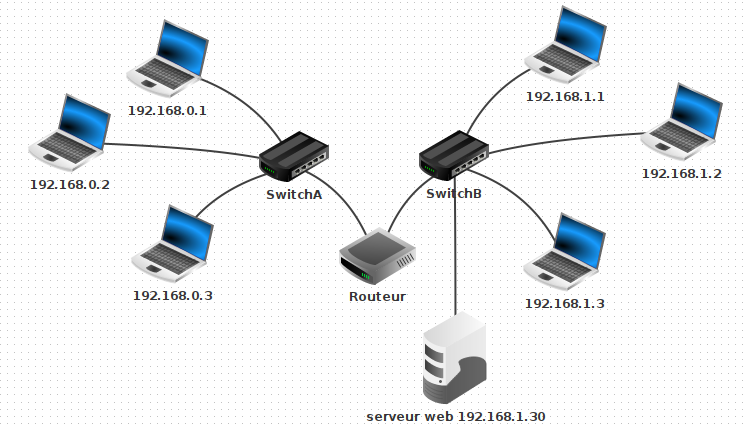
\includegraphics[width=12cm]{img/serveurweb.png}
      \end{center}

    \item Démarrer le serveur web.
    \item Ajouter un navigateur web sur la machine \texttt{192.168.0.1}.
    \item Taper l'adresse IP du serveur web dans la barre d'adresse du navigateur.

      \begin{center}
	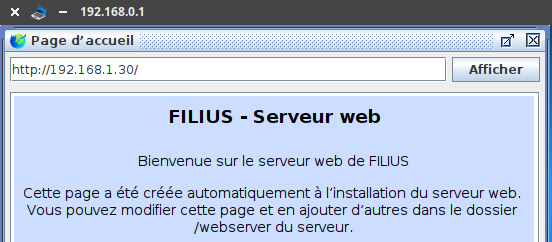
\includegraphics[width=12cm]{img/nav1.png}
      \end{center}
  \end{enumerate}
\end{activite}

\medskip

\begin{activite}[breakable]{serveur DNS}{}
  Lors d'une utilisation classique d'un navigateur web, c'est une url mémorisable qui s'affiche, et non une adresse IP : on retient en effet plus facilement \url{https://www.google.com/} que\\ \url{http://216.58.213.131}, qui renvoient pourtant à la même adresse.

  \smallskip

  La machine qui assure ce rôle d'annuaire entre les serveurs web et leur adresse IP s'appelle un {\color{red}serveur DNS}. Pour pouvoir indexer la totalité des sites internet, son rôle est structuré de manière hiérarchique.

  \begin{enumerate}
    \item Ajouter un serveur DNS minimal, qui n'aura dans son annuaire qu'un seul site. Il faut pour cela raccorder une nouvelle machine (mais une machine déjà sur le réseau aurait très bien pu jouer ce rôle) et y installer un server DNS.

      \begin{center}
	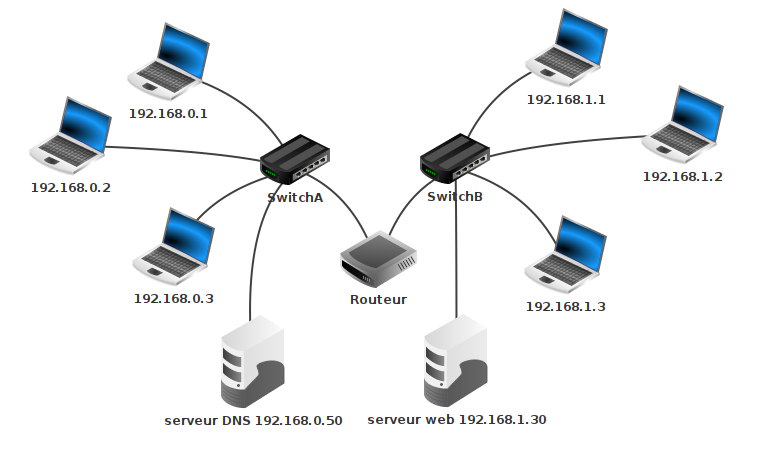
\includegraphics[width=12cm]{img/dns.png}
      \end{center}

    \item Sur ce serveur DNS, associer l'adresse \url{http://www.vivelansi.fr} à l'adresse IP \texttt{192.168.1.30}.

      \begin{center}
	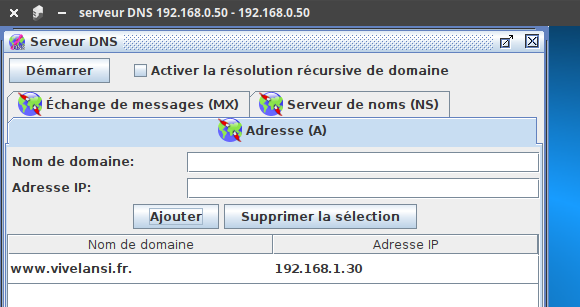
\includegraphics[width=8cm]{img/vivelansi.png}
      \end{center}

    \item Sur la machine \texttt{192.168.0.1}, spécifier l'adresse du serveur DNS :

      \begin{center}
	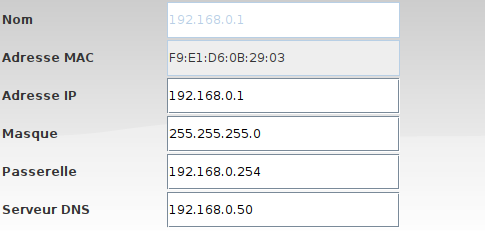
\includegraphics[width=8cm]{img/specdns.png}
      \end{center}

    \item Dans la barre d'adresse du navigateur (de la machine \texttt{192.168.0.1}), essayer l'adresse \\\url{http://www.vivelansi.fr}.

      \begin{center}
	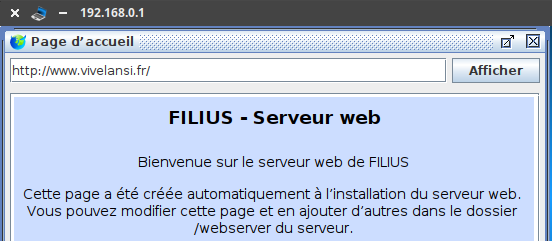
\includegraphics[width=8cm]{img/dnsex.png}
      \end{center}
  \end{enumerate}
\end{activite}

\section{Le modèle en couches}

\subsection{Découpage des données en paquets}

Dans un réseau informatique, si on veut transmettre une image de plusieurs mégaoctets, on n'envoie pas les données en un seul bloc mais on les découpe en paquets plus petits qui sont transmis séparément. Ainsi, il n'est pas nécessaire de tout retransmettre en cas d'erreur. De plus cela réduit les risques d'encombrement ou de blocage des liens.

\subsection{Modèle en couches et encapsulation des données}

\begin{exercice}{}{}
  \begin{enumerate}
    \item Regarder la vidéo disponible \href{https://www.youtube.com/watch?v=26jazyc7VNk}{ici}.
    \item Quel est le principe de l'encapsulation des données dans un réseau informatique ?
      \begin{enumerate}
	\item Cacher les données afin que l'on ne puisse pas les lire
	\item Mettre les données les unes à la suite des autres
	\item Inclure les données d'un protocole dans un autre protocole
	\item Chiffrer les données afin que l'on ne puisse pas les lire
      \end{enumerate}
  \end{enumerate}
\end{exercice}

\medskip

Les deux schémas suivants résument cette section :

\begin{center}
  \fbox{
    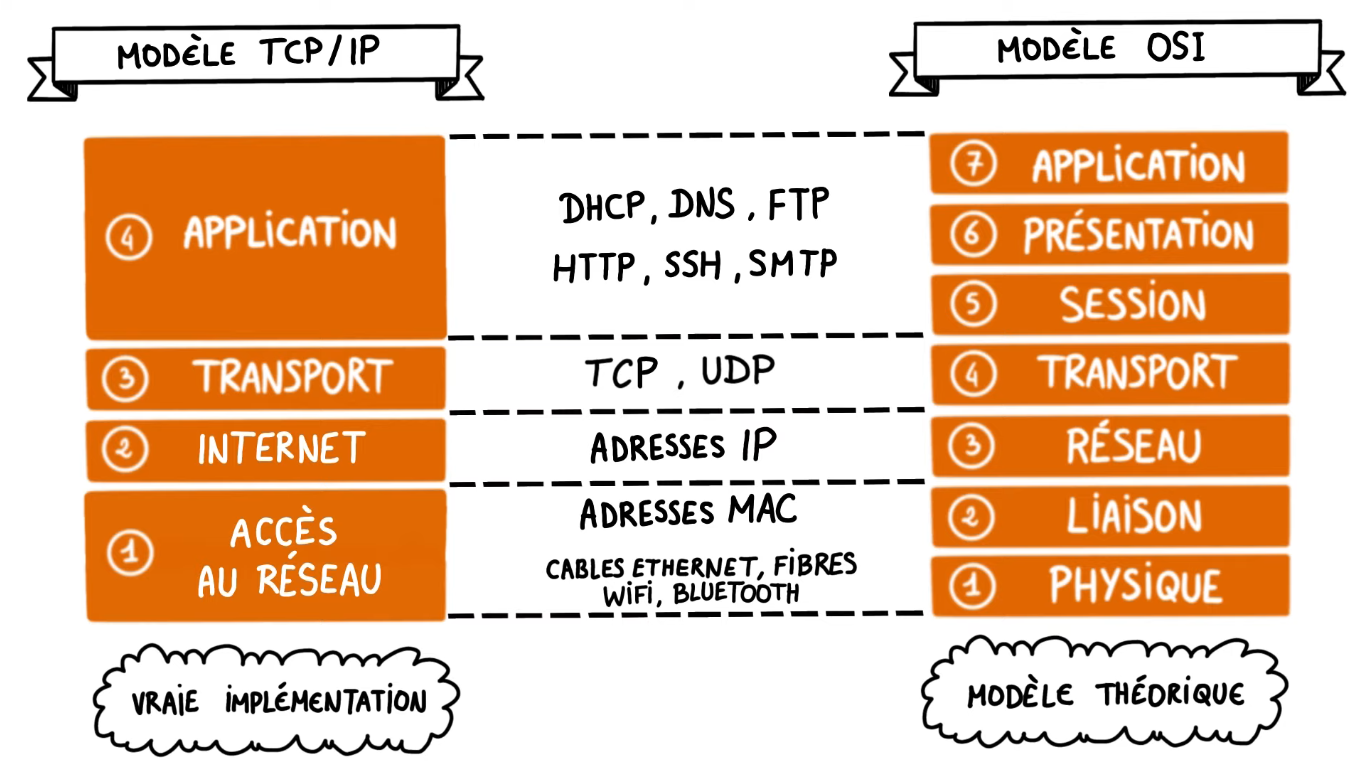
\includegraphics[width=15cm]{img/modeles_tcp_ip_et_osi.png}
  }

  \smallskip

  \scriptsize\textit{Modèles TCP/IP et OSI}
\end{center}

\begin{center}
  \fbox{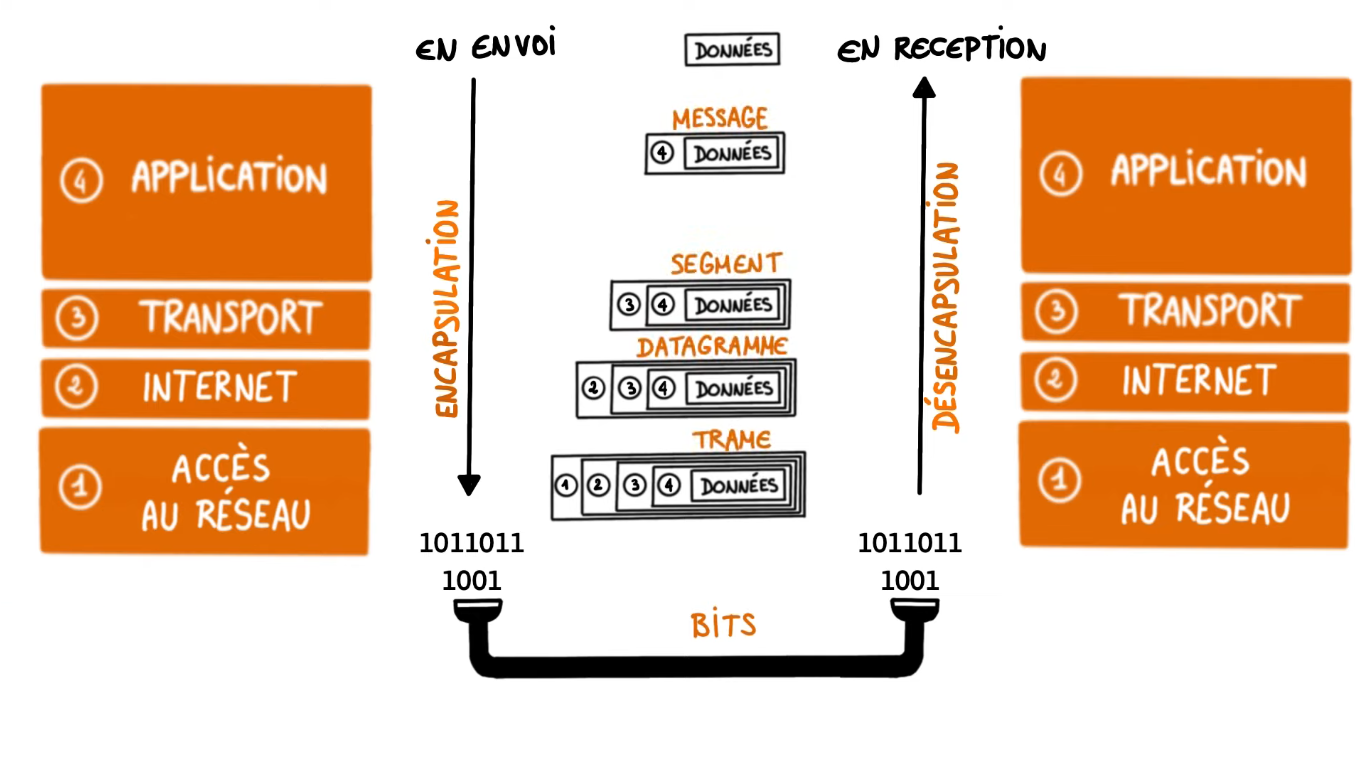
\includegraphics[width=15cm]{img/modele_tcp_ip.png}}

  \smallskip

  \scriptsize\textit{Encapsulation et désencapsulation dans le modèle TCP/IP}
\end{center}

\section{Protocole du bit alterné}

Le protocole du bit alterné est un exemple simple de fiabilisation du transfert de données.

\subsection{Contexte}

\begin{itemize}
  \item Alice veut envoyer à Bob un message \texttt{M}, qu'elle a prédécoupé en sous-messages \texttt{M0}, \texttt{M1}, \texttt{M2}, ...
  \item Alice envoie ses sous-messages à une cadence $\Delta t$ fixée (en pratique, les sous-messages partent quand leur acquittement a été reçu ou qu'on a attendu celui-ci trop longtemps : on parle alors de timeout).
\end{itemize}

\subsection{Situation idéale}

Voici un schéma décrivant la situation idéale dans laquelle tous les sous-messages arrivent à destination, dans le bon ordre.

\begin{center}
  \fbox{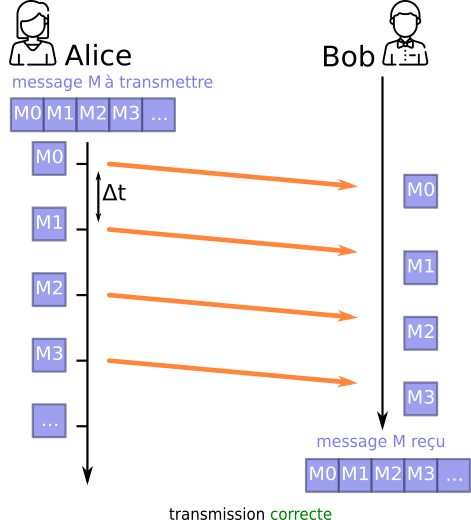
\includegraphics[width=9cm]{img/ideale.png}}
\end{center}

\subsection{Situation réelle}

Mais parfois, les choses ne se passent pas toujours aussi bien car si on maîtrise parfaitement le timing de l'envoi des sous-messages d'Alice, on ne sait pas combien de temps vont mettre ces sous-messages pour arriver, ni même s'ils ne vont pas être détruits en route.

\begin{center}
  \fbox{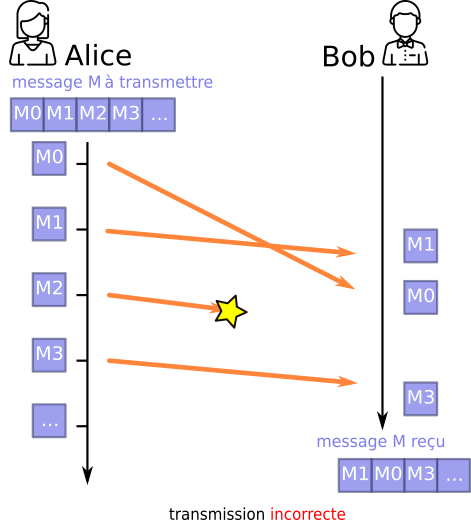
\includegraphics[width=9cm]{img/realite.png}}
\end{center}

Le sous-message \texttt{M0} est arrivé après le \texttt{M1}, le message \texttt{M2} n'est jamais arrivé...

Numéroter les sous-messages afin que Bob puisse les remettre dans l'ordre ou redemander spécifiquement les sous-messages perdus est coûteux en ressources. Il existe une solution plus basique.

\subsection{Idée naïve}

Une idée naïve consiste de demander à Bob d'envoyer un signal pour dire à Alice qu'il vient bien de recevoir son sous-message. On appellera ce signal ACK (comme acknowledgement, traduisible par \og{}accusé de réception\fg{}). Ce signal ACK permettra à Alice de renvoyer un message qu'elle considèrera comme perdu :

\begin{center}
  \fbox{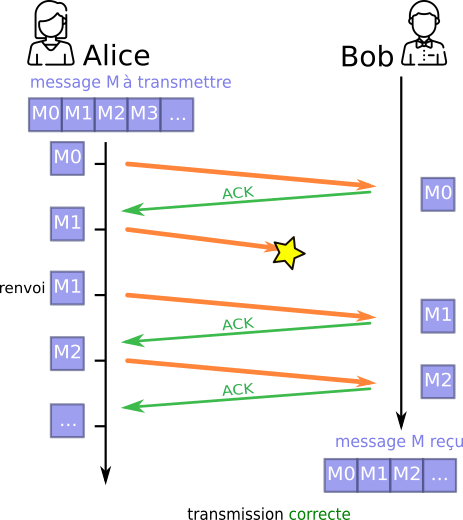
\includegraphics[width=9cm]{img/naive.png}}
\end{center}

\begin{exercice}{}{}
  Décrire la situation précédente.
  % correction
  % N'ayant pas reçu le ACK consécutif à son message \texttt{M1}, Alice suppose (avec raison) que ce message n'est pas parvenu jusqu'à Bob, et donc renvoie le message \texttt{M1}.
\end{exercice}

\begin{exercice}{}{}
  Expliquer pourquoi la solution décrite précédemment n'est pas suffisante à l'aide du schéma ci-dessous :
  \begin{center}
    \fbox{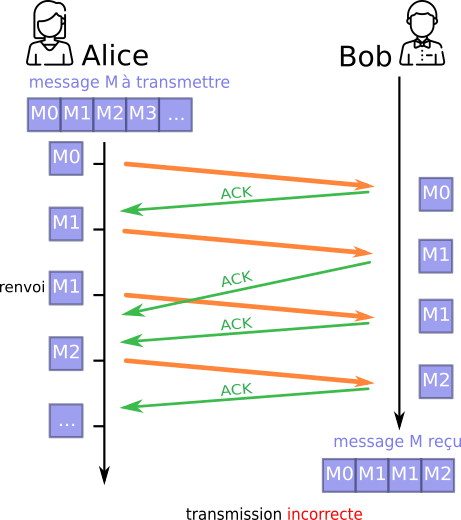
\includegraphics[width=9cm]{img/naivebad.png}}
  \end{center}
  % correction
  % Le deuxième ACK de Bob a mis trop de temps pour arriver (ou s'est perdu en route) et donc Alice a supposé que son sous-message \texttt{M1} n'était pas arrivé. Elle l'a donc renvoyé, et Bob se retrouve avec deux fois le sous-message \texttt{M1}. La transmission est incorrecte. En faisant transiter un message entre Bob et Alice, nous multiplions par 2 la probabilité que des problèmes techniques de transmission interviennent. Et pour l'instant rien ne nous permet de les détecter.
\end{exercice}

\subsection{Protocole du bit alterné}

\begin{definition}[breakable, title=Description du protocole]{}{}
  Bob va maintenant intégrer une méthode de validation du sous-message reçu. Il pourra décider de le garder ou de l'écarter. Le but est d'éviter les doublons.

  \smallskip

  Pour réaliser ceci, Alice va rajouter à chacun de ses sous-messages un bit de contrôle, qu'on appelera FLAG (drapeau). Au départ, ce FLAG vaut 0. Quand Bob reçoit un FLAG, il renvoie un ACK égal au FLAG reçu.

  \smallskip

  Alice va attendre cet ACK contenant le même bit que son dernier FLAG envoyé :

  \begin{itemize}
    \item tant qu'elle ne l'aura pas reçu, elle continuera à envoyer le même sous-message, avec le même FLAG ;
    \item dès qu'elle l'a reçu, elle peut envoyer un nouveau sous-message en inversant (\og{}alternant\fg{}) le bit de son dernier FLAG (d'où le nom de ce protocole).
  \end{itemize}

  Bob, de son côté, va contrôler la validité de ce qu'il reçoit : il ne gardera que les sous-messages dont le FLAG est égal à l'inverse de son dernier ACK. C'est cette méthode qui lui permettra d'écarter les doublons.
\end{definition}

\medskip

\begin{exercice}[breakable]{}{}

  Observer le protocole du bit alterné dans les trois cas ci-dessous et expliquer pourquoi la transmission est correcte.

  \begin{center}
    \fbox{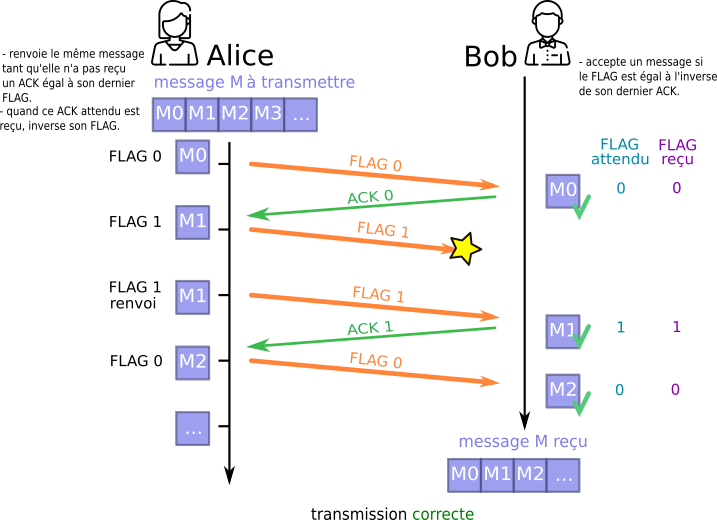
\includegraphics[width=14cm]{img/alt2.png}}
  \end{center}

  \begin{center}
    \fbox{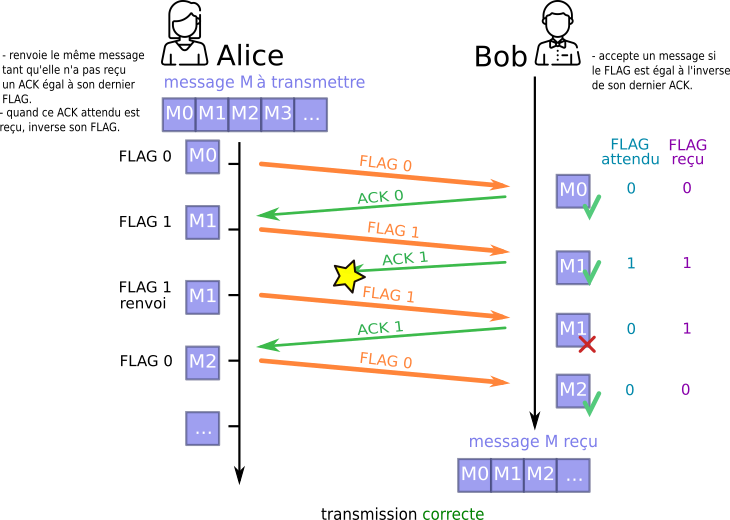
\includegraphics[width=14cm]{img/alt1.png}}
  \end{center}

  \begin{center}
    \fbox{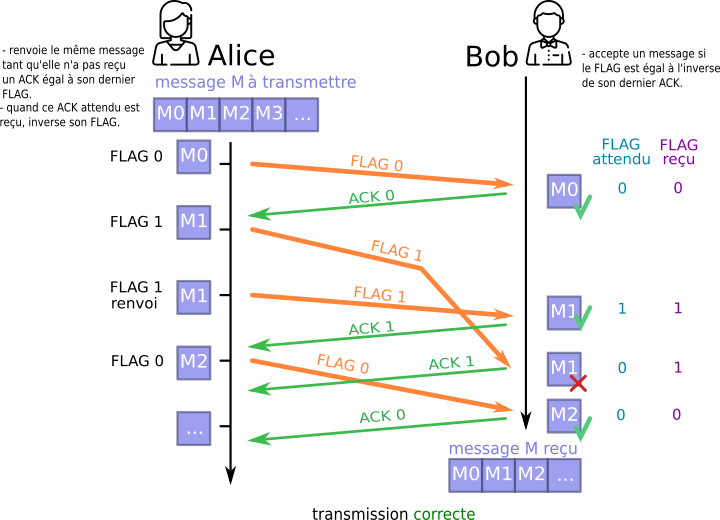
\includegraphics[width=14cm]{img/alt3.png}}
  \end{center}
\end{exercice}

\subsection{Conclusion}

Le protocole du bit alterné a longtemps été utilisé au sein de la couche 2 du modèle OSI (distribution des trames Ethernet). Simple et léger, il peut toutefois être facilement mis en défaut, ce qui explique qu'il ait été remplacé par des protocoles plus performants.
\end{document}
